% !TeX spellcheck = en_GB
\documentclass[10pt]{beamer}
\usetheme{CambridgeUS}
%\usetheme{Boadilla}
\definecolor{myred}{RGB}{163,0,0}
%\usecolortheme[named=blue]{structure}
\usecolortheme{dove}
\usefonttheme[]{professionalfonts}
\usepackage[english]{babel}
\usepackage{amsmath,amsfonts,amssymb}
\usepackage{xcolor}
\usepackage{bm}
\usepackage{gensymb}
\usepackage{verbatim} 
\usepackage{paratype}
\usepackage{mathpazo}
\usepackage{listings}
\lstset{language=Python}

\usepackage{tikz}
\usetikzlibrary{matrix}

\DeclareMathOperator*{\interior}{int}

% Number theorem environments
\setbeamertemplate{theorem}[ams style]
\setbeamertemplate{theorems}[numbered]

% Reset theorem-like environments so that each is numbered separately
\usepackage{etoolbox}
\undef{\definition}
\theoremstyle{definition}
\newtheorem{definition}{\translate{Definition}}
\newtheorem{Fact}{\translate{Fact}}

% Change colours for theorem-like environments
\definecolor{mygreen1}{RGB}{0,96,0}
\definecolor{mygreen2}{RGB}{229,239,229}
\setbeamercolor{block title}{fg=white,bg=mygreen1}
\setbeamercolor{block body}{fg=black,bg=mygreen2}



\alt<presentation>
{\lstset{%
  basicstyle=\footnotesize\ttfamily,
  commentstyle=\slshape\color{green!50!black},
  frame = single,  
  keywordstyle=\bfseries\color{blue!50!black},
  identifierstyle=\color{blue},
  stringstyle=\color{orange},
  %escapechar=\#,
  showstringspaces = false,
  showtabs = false,
  tabsize = 2,
  emphstyle=\color{red}}
}
{
  \lstset{%
    basicstyle=\ttfamily,
    keywordstyle=\bfseries,
    commentstyle=\itshape,
    escapechar=\#,
    showtabs = false,
	tabsize = 2,
    emphstyle=\bfseries\color{red}
  }
} 

\title{R401: Statistical and Mathematical Foundations}
\subtitle{Lecture 15: Nonlinear Programming and Concave Optimization}
\author{Andrey Vassilev}

\date{2016/2017} 
    
\AtBeginSection{\frame{\usebeamerfont{section title}\centering\insertsection}}

\begin{document}
\maketitle



\begin{frame}[fragile]
\frametitle{Lecture Contents}
\tableofcontents
\end{frame}

\begin{section}{Static optimization with inequality constraints}\label{sec:ineq}

\begin{frame}[fragile]
\frametitle{Basic formulation with inequality constraints}
We now look at a problem which is very similar to the case of optimization with equality constraints:

\begin{equation}
f(x_1,\ldots,x_n)\rightarrow \max 
\label{eq:obj}
\end{equation}
s.t.
\begin{equation}
\begin{array}{l l l}
g_1(x_1,\ldots,x_n) \leq b_1\\
g_2(x_1,\ldots,x_n) \leq b_2\\
\cdots \\
g_m(x_1,\ldots,x_n) \leq b_m\\
\end{array}.
\label{eq:constr}
\end{equation}
In vector notation:
\[ f(\mathbf{x}) \rightarrow \max \]
s.t. \[ \mathbf{g}(\mathbf{x})\leq \mathbf{b}. \]
\end{frame}

\begin{frame}[fragile]
\frametitle{Basic formulation with inequality constraints}
\begin{itemize}
\item A vector $ \mathbf{x} $ satisfying the constraints \eqref{eq:constr} is called \emph{admissible} or \emph{feasible}.\bigskip
\item In some alternative (but essentially equivalent) formulations the constraints take the form
$ g_i(x_1,\ldots,x_n)\leq 0 $ or $ g_i(x_1,\ldots,x_n)\geq 0 $ for $ i=1,\ldots,m $.\bigskip
\item The set of admissible vectors is called the \emph{admissible (feasible) set}.\bigskip
\item With inequality constraints the requirement $ m<n $ is not necessary. Intuitively, this is because an inequality constraint is much more forgiving: think of a line vs. a half-plane.\bigskip
\item We focus on maximization problems here. Notice that minimizing a function $ f(x) $ is equivalent to maximizing $ -f(x) $, so there is no loss of generality in our choice.
\end{itemize}
\end{frame}

\begin{frame}[fragile]
\frametitle{Basic formulation with inequality constraints}
\framesubtitle{The Lagrangian}
We again approach problem \eqref{eq:obj}-\eqref{eq:constr} by defining a \emph{Lagrangian}:

\[ \mathcal{L}(\mathbf{x}) = f(\mathbf{x}) - \lambda_1 (g_1(\mathbf{x})-b_1) - \cdots - \lambda_m (g_m(\mathbf{x})-b_m). \]\bigskip

The Lagrangian takes the familiar form from the case of equality constraints! \bigskip

The differences arise in the algorithm used to obtain candidates for optimality.
\end{frame}

\begin{frame}[fragile]
\frametitle{Solution recipe for the case of inequality constraints}
When trying to find solutions to \eqref{eq:obj}-\eqref{eq:constr}, the following procedure is often applied:

\begin{block}{Algorithm (Kuhn-Tucker conditions)}
\begin{enumerate}
\item Form the Lagrangian
\item Differentiate it w.r.t. the elements of $ \mathbf{x} $ and set the resulting derivatives equal to zero:
\begin{equation}
\dfrac{\partial \mathcal{L}}{\partial x_i} = \dfrac{\partial f(\mathbf{x})}{\partial x_i} - \sum_{j=1}^{m}\lambda_j \dfrac{\partial g_j(\mathbf{x})}{\partial x_i} = 0,~i=1,\ldots,n.
\label{eq:dLdX}
\end{equation}
\item Check the \emph{complementary slackness} conditions \begin{equation}
\lambda_j \geq 0 \text{ and } \lambda_j (g_j(\mathbf{x})-b_j) = 0,~j=1,\ldots,m.
\label{eq:ComplSlack}
\end{equation}
\item The points satisfying 2) and 3) above are the candidates for optimality
\end{enumerate}
\end{block}

Condition 3) above implies that \[ \lambda_j = 0 \text{ if } g_j(\mathbf{x})<b_j,~j=1,\ldots,m. \]
\end{frame}

\begin{frame}[fragile]
\frametitle{Comments on the Kuhn-Tucker conditions}
\begin{itemize}
\item The term \emph{complementary slackness} derives from the fact that according to \eqref{eq:ComplSlack} one of the conditions $ \lambda_j \geq 0 $ and $ g_j(x_1,\ldots,x_n) \leq b_j $ may be \emph{slack} (i.e. be a strict inequality), while the other must bind (i.e. be fulfilled as an equality). Thus, they \emph{complement} each other. \bigskip
\item Let $ \mathbf{x^*} $ be an admissible point. If it is true that $ g_j(\mathbf{x^*})=b_j $, the respective constraint is called \emph{active} or \emph{binding}. \bigskip
\item It is possible to have simultaneously $ \lambda_j = 0 $ and $ g_j(\mathbf{x^*})=b_j $ for some $ j $s. 
\end{itemize}
\end{frame}

\begin{frame}[fragile]
\frametitle{A simple illustration of the Kuhn-Tucker procedure}
\begin{example}
\[ \max_{x,y} f(x,y) = xy \]
s.t. \[ x^2+y^2 \leq 1. \]

The Lagrangian is
\[ \mathcal{L} = xy - \lambda (x^2+y^2-1). \]
\[ \dfrac{\partial \mathcal{L}}{\partial x} = y-2\lambda x=0 \quad \Rightarrow \quad y = 2\lambda x, \]
\[ \dfrac{\partial \mathcal{L}}{\partial y} = x-2\lambda y=0 \quad \Rightarrow \quad x = 2\lambda y. \]

The complementary slackness condition reads \[ \lambda (x^2+y^2-1)=0. \]
\label{ex:KTillustrated}
\end{example}
\end{frame}

\begin{frame}[fragile]
\frametitle{A simple illustration of the Kuhn-Tucker procedure}\addtocounter{theorem}{-1}
\begin{example}[cont.]
Assume $ \lambda = 0 $. Then the conditions $ \frac{\partial \mathcal{L}}{\partial x}=\frac{\partial \mathcal{L}}{\partial y}=0 $ imply $ x=y=0$, which provides one candidate.\bigskip

Assume $ \lambda \neq 0 $. We have $ x^2+y^2 = 1 $. Note that $ x=0 $ would imply $ y=0 $ and vice versa, which would violate the condition $ x^2+y^2 = 1 $. Thus, $ x,y \neq 0 $. Then we obtain \[ \dfrac{x}{y}=\dfrac{y}{x} \quad \Rightarrow \quad x^2 = y^2. \]\bigskip
\end{example}
\end{frame}

\begin{frame}[fragile]
\frametitle{A simple illustration of the Kuhn-Tucker procedure}\addtocounter{theorem}{-1}
\begin{example}[cont.]
The result $ x^2 = y^2 $, combined with $ x^2+y^2 = 1 $, yields four possibilities: \[ \begin{array}{l l l l l l r}
(x,y) & = & \left(\frac{1}{\sqrt{2}},\frac{1}{\sqrt{2}}\right) & \Rightarrow & \lambda &=& \frac{1}{2},\\
(x,y) & = & \left(-\frac{1}{\sqrt{2}},\frac{1}{\sqrt{2}}\right)& \Rightarrow &\lambda &=& -\frac{1}{2},\\
(x,y) & = & \left(\frac{1}{\sqrt{2}},-\frac{1}{\sqrt{2}}\right)& \Rightarrow &\lambda &=& -\frac{1}{2},\\
(x,y) & = & \left(-\frac{1}{\sqrt{2}},-\frac{1}{\sqrt{2}}\right)& \Rightarrow &\lambda &=& \frac{1}{2} .
\end{array} \]

The second and third case can be excluded, as they are associated with $ \lambda<0 $. Thus, we are left with the candidates $ x=y=\frac{1}{\sqrt{2}} $ and $ x=y=-\frac{1}{\sqrt{2}} $ in addition to the candidate $ x=y=0$ obtained above. Note, however, that the last point yields a smaller value of the objective function and can be excluded.
\end{example}
\end{frame}

\begin{frame}[fragile]
\frametitle{From the Kuhn-Tucker algorithm to necessary conditions}
While the Kuhn-Tucker algorithm in its present form provides us with candidates, we need to strengthen it further to obtain proper necessary conditions for optimality.\pause

\begin{Fact}[Kuhn-Tucker necessary conditions]
Let $ \mathbf{x^*}=(x_1^*,\ldots,x_n^*)' $ be a solution to \eqref{eq:obj}-\eqref{eq:constr}. Suppose that the functions $ f $ and $ g_i,~i=1,\ldots,m ,$ have continuous partial derivatives on a set $ S\subseteq \mathbb{R}^n $, and $ \mathbf{x^*} \in \interior S $. Suppose also that the gradients of the constraints which are binding at $ \mathbf{x^*} $, are linearly independent, i.e. if $ K := \{k~\vert~ g_k(\mathbf{x^*})=0\} $, it is true that \[ \nabla g_k(\mathbf{x^*}),~k\in K, \text{ are linearly independent.} \]

Then there exist unique numbers $ \lambda_1^*,\ldots,\lambda_m^* $ such that equations \eqref{eq:dLdX} and \eqref{eq:ComplSlack} hold at $ \mathbf{x^*} $.
\label{fc:KT_NCs}
\end{Fact}\bigskip

The linear independence condition in Fact \ref{fc:KT_NCs} is called the \emph{constraint qualification (CQ)}.
\end{frame}

\begin{frame}[fragile]
\frametitle{An equivalent formulation of the constraint qualification}
Take the \emph{Jacobian} of the constraint function $ \mathbf{g}(\mathbf{x}) $ and remove the rows that correspond to the inactive constraints:
\[ 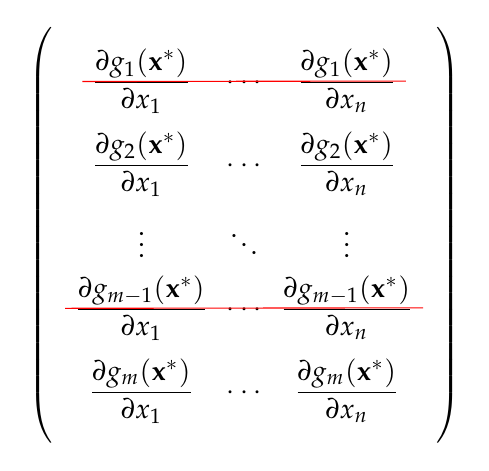
\begin{tikzpicture}
     \matrix (mat)[matrix of math nodes,left delimiter={(},right delimiter={)}]
      {%
		\dfrac{\partial g_1 (\mathbf{x^*})}{\partial x_1}  &  \cdots  &  \dfrac{\partial g_1 (\mathbf{x^*})}{\partial x_n} \\
		\dfrac{\partial g_2 (\mathbf{x^*})}{\partial x_1}  &  \cdots  &  \dfrac{\partial g_2 (\mathbf{x^*})}{\partial x_n} \\
		\vdots   &  \ddots  &  \vdots \\
		\dfrac{\partial g_{m-1} (\mathbf{x^*})}{\partial x_1}  &  \cdots  &  \dfrac{\partial g_{m-1} (\mathbf{x^*})}{\partial x_n} \\
		\dfrac{\partial g_{m} (\mathbf{x^*})}{\partial x_1}  &  \cdots  &  \dfrac{\partial g_{m} (\mathbf{x^*})}{\partial x_n} \\
      }; \pause
      \draw[red](mat-1-1.west) -- (mat-1-3.east);
      \draw[red](mat-4-1.west) -- (mat-4-3.east);
\end{tikzpicture}
\]

\uncover<3->{Here the first and the $ (m-1) $-th constraints are \textbf{not} binding.}
\end{frame}

\begin{frame}[fragile]
\frametitle{An equivalent formulation of the constraint qualification}
Thus, if $ k $ out of $ m $ constraints are not binding, we are left with a $ (m-k)\times n $ matrix of partial derivatives, evaluated at $ \mathbf{x^*} $.\bigskip

The constraint qualification requires that the rank of this matrix should be equal to the number of rows $ m-k $.\bigskip \bigskip

\textbf{Remark:} While we work with a specific version of the CQ here, bear in mind that the term ``constraint qualification'' refers to a whole class of different regularity conditions used in optimization problems.
\end{frame}

\begin{frame}[fragile]
\frametitle{Applying the necessary conditions}
The CQ is a potential source of problems when applying the Kuhn-Tucker necessary conditions: it is possible to have an optimal point where the CQ (and hence the NCs) fail. \bigskip


Therefore the general procedure is as follows:
\begin{enumerate}
\item Use Fact \ref{fc:KT_NCs} to find a set of candidates.
\item Find the feasible points where the CQ fails. These are also candidates.
\item Search for the optimum over the union of the preceding two sets.
\end{enumerate}\bigskip

For more complicated problems one approach is to work over the various combinations of constraints (assume all are binding, one is binding etc.) and to study these cases one by one.
\end{frame}

\begin{frame}[fragile]
\frametitle{Some illustrations}
\begin{example}[Example \ref{ex:KTillustrated} revisited]
The solution of Example \ref{ex:KTillustrated} did not make use of the CQ condition. Let us check it now: \[ g(x,y)=x^2+y^2 \quad \Rightarrow \quad \nabla g(x,y) = (2x,2y)'. \]

Since any single vector except the zero vector is linearly independent in itself, the CQ fails only at $ (0,0)' $.

Therefore, a strict application of Fact \ref{fc:KT_NCs} would have required to treat the case $ x=0,~y=0 $ separately, to establish the other two possibilities $ x=y=\frac{1}{\sqrt{2}} $ and $ x=y=-\frac{1}{\sqrt{2}} $, and then to compare the three cases. In working through Example  \ref{ex:KTillustrated} we obtained the first case via the K-T algorithm.
\label{ex:revisitKTillustrated}
\end{example}\bigskip

\textbf{Homework:} Consider the problem $ \max_{x,y} f(x,y)=1-2x^2-3y^2 $ s.t. $ x\geq 5,~y \geq 6 $. Solve it using the K-T procedure. Can you guess the solution without using formal methods?
\end{frame}

\begin{frame}[fragile]
\frametitle{Some illustrations}
\begin{example}
Consider the problem
\[ f(x_1,x_2) = -x_1^3+x_2 \rightarrow \max \]
s.t. \[ x_2\leq 0. \]

We have \[ \mathcal{L} =  -x_1^3+x_2 - \lambda x_2  \]
\[ \dfrac{\partial \mathcal{L}}{\partial x_1} = -3x_1^2 = 0 \quad \Rightarrow \quad x_1 = 0. \]
\[ \dfrac{\partial \mathcal{L}}{\partial x_2} = 1-\lambda = 0 \quad \Rightarrow \quad \lambda = 1. \]

Complementary slackness requires that $ \lambda x_2 = 0 $, hence $ x_2 = 0 $.
\label{ex:KTfail}
\end{example}
\end{frame}

\begin{frame}[fragile]
\frametitle{Some illustrations}\addtocounter{theorem}{-1}
\begin{example}[cont.]
The gradient of the constraint function is $\nabla g(x_1,x_2) = (g'_x(x_1,x_2),g'_y(x_1,x_2))' = (0,1)' $, so the CQ is satisfied everywhere. \bigskip

To sum up, the K-T NCs are satisfied and $ x_1=0,~x_2=0 $ is our only candidate.\bigskip

However, it is easily seen that any point of the type $ (x_1,0) $ with $ x_1<0 $ is admissible, and for $ x_1 \rightarrow -\infty $ the objective function grows unboundedly. 

This again illustrates the need to use NCs with caution. 
\end{example}
\end{frame}


\begin{frame}[fragile]
\frametitle{Sufficient conditions}
The following fact provides a sufficient condition for optimality by imposing a concavity requirement on the Lagrangian.

\begin{Fact}
Let $ \mathbf{x^*} $ be an admissible point for the problem \eqref{eq:obj}-\eqref{eq:constr}. 

Suppose that:\begin{enumerate}
\item We can find a vector $ (\lambda_1^*,\ldots,\lambda_m^*)' $ which, together with $ \mathbf{x^*} $, satisfies equations \eqref{eq:dLdX} and \eqref{eq:ComplSlack} in the K-T algorithm .
\item The Lagrangian is concave.
\end{enumerate}

Then the point $ \mathbf{x^*} $ is optimal.
\label{fc:SCsIneq}
\end{Fact}
\end{frame}


\begin{frame}[fragile]
\frametitle{Sufficient conditions}
\framesubtitle{Remarks}
\begin{itemize}
\item The requirement of concavity or convexity of a Lagrangian or a similar object is a popular way of obtaining sufficient conditions for optimality.
\item Rather than working directly with the definition of concavity, it is often useful to apply special results to show concavity. Examples include:
\begin{itemize}
\item The sum of concave functions is concave.
\begin{itemize}
\item As a special case, if $ f(x_1,\ldots,x_n)=\sum_{i=1}^{n}f_i(x_i) $ and $ f_i $ are concave, then $ f $ is also concave.
\end{itemize}
\item If $ f $ is concave and $ \alpha>0 $, then $ \alpha f $ is concave.
\item A twice differentiable function of one variable is concave on an interval $ I $ if $ f''(x)\leq 0, ~\forall x \in I $.
\item Let $ f(\mathbf{x}) $ be a twice differentiable function defined on an open convex set $ S\subset \mathbb{R}^n $. The function $ f(\mathbf{x}) $ is concave in $ S $ if and only if the Hessian $ \mathbf{f''(x)} $ is negative semidefinite for all $ \mathbf{x}\in S $. If the Hessian $ \mathbf{f''(x)} $ is negative definite for all $ \mathbf{x}\in S $, it follows that $ f(\mathbf{x}) $ is \emph{strictly} concave in $ S $.
\end{itemize}
\item Similar results hold for convex functions. See SHSS, 2.2-2.4, for more information on convex sets and concave/convex functions.
\end{itemize}
\end{frame}

\begin{frame}[fragile]
\frametitle{Example: utility maximization}
Consider a consumer with income $ I $ who plans to buy certain quantities, $ x_1 $ and $ x_2 $, of two goods at prices $ p_1 $ and $ p_2 $, respectively . Obviously, we require $ p_1,p_2,I >0 $. The consumer's preferences are described via the utility function \[ U(x_1,x_2) = x_1^\alpha x_2^\beta,\quad \alpha,\beta >0,~\alpha+\beta < 1. \] 

The consumer's feasible set is characterized by the budget constraint and nonnegativity constraints on the quantities:   \[ p_1 x_1 + p_2 x_2 \leq I , \]  
\[ x_1\geq 0 , \] \[ x_2 \geq 0. \] 

The consumer seeks to maximise utility subject to the above constraints.
\end{frame}

\begin{frame}[fragile]
\frametitle{Example: utility maximization}
Notice that the consumer is \textbf{not} required to spend all his income!\bigskip

To cast the problem in canonical form, we rewrite the nonnegativity constraints as
\[ -x_1\leq 0 , \qquad -x_2 \leq 0. \] \bigskip

The Lagrangian is \[ \mathcal{L} = x_1^\alpha x_2^\beta - \lambda_1 ( p_1 x_1 + p_2 x_2 - I) -\lambda_2 (-x_1) - \lambda_3 (-x_2) \] and is {\color{red}concave} in $ (x_1,x_2) $.\bigskip

\textbf{Homework:} Prove the concavity of $ \mathcal{L} $.\bigskip

\textbf{Note: }The concavity of the Lagrangian depends on the concavity of $ U(x_1,x_2) $, which hinges on the assumption $ \alpha+\beta < 1 $.
\end{frame}

\begin{frame}[fragile]
\frametitle{Example: utility maximization}
\begin{figure}
\centering
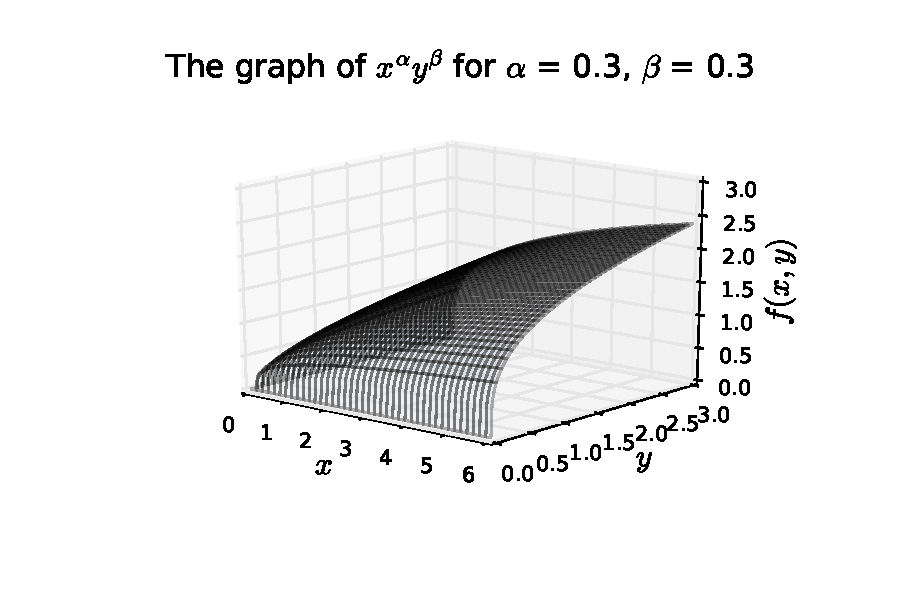
\includegraphics[width=0.5\linewidth]{ConcF}
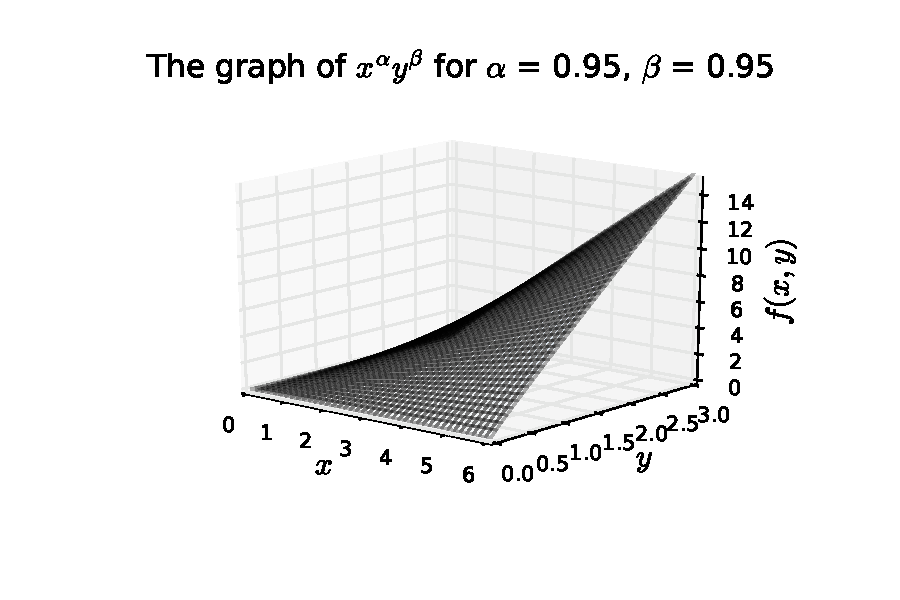
\includegraphics[width=0.5\linewidth]{NonConcF}
\end{figure}
\end{frame}

\begin{frame}[fragile]
\frametitle{Example: utility maximization}
Notice that the Lagrangian is not differentiable at $ x_1=0 $ or $ x_2=0 $. However, we can exclude those cases as it is immediately seen that any feasible point with positive elements yields a positive value of the utility function (compared to the zero utility when one or both $ x_i $ is zero).\bigskip

Then, we can apply the K-T algorithm:\begin{align*}
&\dfrac{\partial \mathcal{L}}{\partial x_1} = \alpha x_1^{\alpha-1} x_2^\beta -\lambda_1 p_1 + \lambda_2 = 0, \\[4pt]
&\dfrac{\partial \mathcal{L}}{\partial x_2} = \beta x_1^\alpha x_2^{\beta-1} -\lambda_1 p_2 + \lambda_3 = 0, \\[4pt]
&\lambda_1 \geq 0, \quad \lambda_1 ( p_1 x_1 + p_2 x_2 - I) = 0, \\[4pt]
&\lambda_2 \geq 0, \quad \lambda_2 x_1 = 0, \\[4pt]
&\lambda_3 \geq 0, \quad \lambda_3 x_2 = 0. 
\end{align*}
\end{frame}

\begin{frame}[fragile]
\frametitle{Example: utility maximization}
We will work through the various possibilities for the Lagrange multipliers. 

These are:

\begin{center}
\begin{tabular}{|c|c|c|c|}
\hline 
Case & $ \lambda_1 $ & $ \lambda_2 $ & $ \lambda_3 $ \\ 
\hline 
1 & 0 & 0 & 0 \\ 
\hline 
2 & 0 & 0 & + \\ 
\hline 
3 & 0 & + & 0 \\ 
\hline 
4 & 0 & + & + \\ 
\hline 
5 & + & + & + \\ 
\hline 
6 & + & 0 & + \\ 
\hline 
7 & + & + & 0 \\ 
\hline 
8 & + & 0 & 0 \\ 
\hline 
\end{tabular} \end{center}
\end{frame}

\begin{frame}[fragile]
\frametitle{Example: utility maximization}
Our task is made easy by the following observation:\bigskip

If either $ \lambda_2>0 $ or $ \lambda_3>0 $, then the complementary slackness conditions imply $ x_1=0 $ or $ x_2=0 $, which was excluded as a possibility. Thus, we are left to study only Cases 1 and 8.\bigskip

Consider \textbf{Case 1}: $ \lambda_1=\lambda_2=\lambda_3=0 $. The complementary slackness conditions now imply $ x_1,x_2>0 $.

The Lagrangian maximization conditions yield 
\[ \alpha x_1^{\alpha-1} x_2^\beta = 0, \]
\[ \beta x_1^\alpha x_2^{\beta-1} =0, \] which requires that at least one of $ x_1 $ or $ x_2 $ is zero, a contradiction. Therefore, we can disregard this case.
\end{frame}

\begin{frame}[fragile]
\frametitle{Example: utility maximization}
Consider next \textbf{Case 8}: $ \lambda_1>0,~\lambda_2=\lambda_3=0 $. Again the complementary slackness conditions imply $ x_1,x_2>0 $.

The first complementary slackness condition now yields \[ p_1 x_1 + p_2 x_2 = I,  \]
i.e. the budget constraint is binding.

The Lagrangian maximization conditions take the form 
\[ \alpha x_1^{\alpha-1} x_2^\beta -\lambda_1 p_1 = 0, \]
\[ \beta x_1^\alpha x_2^{\beta-1} -\lambda_1 p_2 = 0. \] 

Rearranging these to isolate $ \lambda_1 $ and equating the resulting expressions, we get
\[ \dfrac{\alpha x_1^{\alpha-1}x_2^\beta}{p_1} = \dfrac{\beta x_1^{\alpha}x_2^{\beta-1}}{p_2} \quad \Rightarrow \quad \dfrac{\alpha}{p_1 x_1} = \dfrac{\beta}{p_2 x_2} \quad \Rightarrow \quad x_1 = \dfrac{\alpha p_2}{\beta p_1}x_2. \]
\end{frame}

\begin{frame}[fragile]
\frametitle{Example: utility maximization}
Substitute the expression for $ x_1 $ in the budget constraint: 
\[ p_1 \left(\dfrac{\alpha p_2}{\beta p_1}x_2\right) + p_2 x_2 = I. \]

Solve for $ x_2 $ to obtain \[ x_2 = \dfrac{\beta}{\alpha+\beta}\dfrac{I}{p_2}. \]

Next, substitute the solution for $ x_2 $ in the expression for $ x_1 $ obtained earlier:
\[ x_1 = \dfrac{\alpha p_2}{\beta p_1}\dfrac{\beta}{\alpha+\beta}\dfrac{I}{p_2} \quad \Rightarrow \quad x_1 = \dfrac{\alpha}{\alpha+\beta}\dfrac{I}{p_1}. \]\bigskip

Given that the formulas for $ x_1 $ and $ x_2 $ computed above confirm that $ x_1,x_2>0 $, one can in turn verify that $ \lambda_1 > 0 $.
\end{frame}

\begin{frame}[fragile]
\frametitle{Example: utility maximization}
\framesubtitle{Comments}
\begin{itemize}
\item The above analysis provides \[ x_1 = \dfrac{\alpha}{\alpha+\beta}\dfrac{I}{p_1}, \qquad x_2 = \dfrac{\beta}{\alpha+\beta}\dfrac{I}{p_2} \] as the only K-T candidate. In view of Fact \ref{fc:SCsIneq}, this is the solution to the consumer's problem.
\item The solutions for $ x_1 $ and $ x_2 $ are standard demand functions familiar from microeconomics. The quantities depend negatively on the respective prices and positively on income.
\item We obtained the fact that the budget constraint binds in the course of solving the problem, rather than as an assumption. It was a consequence of having $ \lambda_1 > 0$ in the CS condition. The economic interpretation is that if a resource is valuable (as captured by the fact that its shadow price is positive), then it should not be wasted or left unutilized.
\end{itemize}
\end{frame}

\begin{frame}[fragile]
\frametitle{Wrap up on problems with inequality constraints}
Test your understanding of the material by solving the following:

\textbf{Homework:} \[ \max_{x_1,x_2} 6x_1-2 x_1^2 + 2 x_1 x_2-2x_2^2  \]
s.t. 
\[ 3x_1+4x_2 \leq 6, \] 
\[ -x_1 + 4x_2^2 \leq 2, \]
\[  x_1\geq 0,\quad x_2\geq 0. \]

\textbf{Homework:} A firm produces its output using the production technology $ A q_1^a q_2^b,~a,b>0 $, where $ q_1,q_2 \geq 0 $ are the inputs used in production. The cost per unit of the first input is $ w_1 >0 $ and for the second input is $ w_2 >0$. Demand for the firm's output is $ Q>0 $. Use the K-T approach to find the input combination that minimizes costs while ensuring enough is produced to meet demand, i.e. \[ \min_{q_1,q_2} w_1 q_1 + w_2 q_2\]
s.t. \[ A q_1^a q_2^b \geq Q,\quad q_1,q_2 \geq 0. \]
\end{frame}

\end{section}

\begin{section}{Static optimization with mixed constraints}\label{sec:mixed}

\begin{frame}[fragile]
\frametitle{The case of mixed inequality and equality constraints}
\framesubtitle{Formulation}
Sometimes an optimization problem features a combination of  equality and inequality constraints:

\begin{equation}
f(x_1,\ldots,x_n)\rightarrow \max 
\label{eq:objmx}
\end{equation}
s.t.
\begin{equation}
\begin{array}{l l l}
g_1(x_1,\ldots,x_n) = b_1\\
g_2(x_1,\ldots,x_n) = b_2\\
\cdots \\
g_r(x_1,\ldots,x_n) = b_r\\
h_1(x_1,\ldots,x_n) \leq c_1\\
h_2(x_1,\ldots,x_n) \leq c_2\\
\cdots \\
h_s(x_1,\ldots,x_n) \leq c_s\\
\end{array},
\label{eq:constrmx}
\end{equation}
i.e. \begin{equation*}
\max f(\mathbf{x}) \text{ s.t. } \left\{ \begin{array}{l}
\mathbf{g}(\mathbf{x}) = \mathbf{b}\\
\mathbf{h}(\mathbf{x})\leq \mathbf{c}
\end{array} \right. .
\end{equation*}
\end{frame}

\begin{frame}[fragile]
\frametitle{The case of mixed inequality and equality constraints}
\framesubtitle{Constructing the Lagrangian}
As before, we will require that $ r<n $. \bigskip

The Lagrangian for problem \eqref{eq:objmx}-\eqref{eq:constrmx} is constructed as follows:
\[ \mathcal{L} = f(\mathbf{x}) - \sum_{i=1}^{r}\lambda_i (g_i(\mathbf{x})-b_i) - \sum_{j=1}^{s}\mu_j (h_j(\mathbf{x})-c_j). \]

The Lagrange multipliers conform to the well-known principle: $ \lambda_i $ are free of sign (since they correspond to equality constraints) and $ \mu_j $ must fulfil complementary slackness conditions.
\end{frame}

\begin{frame}[fragile]
\frametitle{Necessary conditions for problems with mixed constraints}
\begin{Fact}
Let $ \mathbf{x^*} $ be a solution to \eqref{eq:objmx}-\eqref{eq:constrmx}. Suppose all functions involved are continuously differentiable and $ r<n $. Suppose further that (without loss of generality) the first $ s_0 $ of the inequality constraints are binding at $ \mathbf{x^*} $ and that the Jacobian comprising those constraints and the equality constraints has rank $ s_0+r $.

Then there exist unique numbers $ \lambda_1^*,\ldots,\lambda_r^* $ and $ \mu_1^*,\ldots,\mu_s^* $ for which \[ \nabla \mathcal{L}(\mathbf{x^*}) = \mathbf{0}, \]
\[ \mu_j^* \geq 0 \text{ and } \mu_j^* (h_j(\mathbf{x^*})-c_j) = 0,~j=1,\ldots,s. \]
\label{fc:Nsmx}
\end{Fact}
\end{frame}

\begin{frame}[fragile]
\frametitle{Necessary conditions for problems with mixed constraints}
In more detail, the Jacobian involving the equality constraints and the active inequality constraints is \[ \begin{pmatrix}
\nabla g_1(\mathbf{x^*})\\
\cdots \\
\nabla g_r(\mathbf{x^*})\\
\nabla h_1(\mathbf{x^*})\\
\cdots \\
\nabla h_{s_0}(\mathbf{x^*})
\end{pmatrix} = \begin{pmatrix}
\dfrac{\partial g_1 (\mathbf{x^*})}{\partial x_1}  &  \cdots  &  \dfrac{\partial g_1 (\mathbf{x^*})}{\partial x_n} \\
\vdots   &  \ddots  &  \vdots \\
\dfrac{\partial g_{r} (\mathbf{x^*})}{\partial x_1}  &  \cdots  &  \dfrac{\partial g_{r} (\mathbf{x^*})}{\partial x_n}\\
\dfrac{\partial h_1 (\mathbf{x^*})}{\partial x_1}  &  \cdots  &  \dfrac{\partial h_1 (\mathbf{x^*})}{\partial x_n} \\
\vdots   &  \ddots  &  \vdots \\
\dfrac{\partial h_{s_0} (\mathbf{x^*})}{\partial x_1}  &  \cdots  &  \dfrac{\partial g_{s_0} (\mathbf{x^*})}{\partial x_n}
\end{pmatrix}. \] 

The requirement on the rank of the Jacobian is the familiar constraint qualification imposing linear independence.
\end{frame}

\begin{frame}[fragile]
\frametitle{Sufficient conditions for problems with mixed constraints}
Analogously to Fact \ref{fc:SCsIneq}, we have the following result for the case of mixed constraints:

\begin{Fact}
Let $ \mathbf{x^*} $ be an admissible point satisfying the conditions stated in Fact \ref{fc:Nsmx}.

Suppose that the Lagrangian for problem \eqref{eq:objmx}-\eqref{eq:constrmx} is concave in $ \mathbf{x} $.\bigskip

Then the point $ \mathbf{x^*} $ is a solution to problem \eqref{eq:objmx}-\eqref{eq:constrmx}.
\label{fc:Scsmx}
\end{Fact}
\end{frame}

\end{section}

\begin{section}{Concave programming}\label{sec:concave}

\begin{frame}[fragile]
\frametitle{Problem description}
Consider the familiar maximization problem with inequality constraints:
\begin{equation}
f(\mathbf{x}) \rightarrow \max
\label{eq:objconc}
\end{equation}
s.t. \begin{equation}
\mathbf{g}(\mathbf{x})\leq \mathbf{b},
\label{eq:constrconc}
\end{equation}
with the additional assumptions that the objective function $ f $ is concave and the functions $ g_i, ~i=1,\ldots,m $, are convex. Then the optimization problem is called a \emph{concave programming problem} or simply a \emph{concave program}.\bigskip

\textbf{Note:} Recall that convex and concave functions are properly defined on \emph{convex} sets (typically convex subsets of $ \mathbb{R}^n $). This is an implicit requirement in the above formulation.
\end{frame}

\begin{frame}[fragile]
\frametitle{The concave case without constraints}
It is useful to start with the following result for \emph{unconstrained} concave optimization problems:
\begin{Fact}
Let $ U $ be a convex subset of $ \mathbb{R}^n $ and $ f $ be a continuously differentiable concave function on $ U $. A point $ \mathbf{x^*} \in U $ is a \emph{global maximum} of $ f $ if and only if \[ \nabla' f(\mathbf{x^*}) (\mathbf{x}-\mathbf{x^*}) \leq 0,\quad \forall \mathbf{x} \in U. \]

If $ U $ is open or $ \mathbf{x^*} \in \interior U$, then $ \mathbf{x^*} $ is a global maximum of $ f $ on $ U $ if and only if \[  \nabla f(\mathbf{x^*}) = 0. \]
\label{fc:ConcaveUnconstr}
\end{Fact}
\end{frame}

\begin{frame}[fragile]
\frametitle{Quasiconcavity and quasiconvexity}
\begin{itemize}
\item Note that for a concave program as defined above the concavity condition on the Lagrangian stated in Fact \ref{fc:SCsIneq} is fulfilled and we can apply Fact \ref{fc:SCsIneq} directly.
\item However, in economic applications it is sometimes useful to generalize the concepts of concave and convex functions and apply them to the concave programming problem as described below.
\item A function $ f $ defined on a convex subset $ U $ of $ \mathbb{R}^n $ is called \emph{quasiconcave} if, for any $ a \in \mathbb{R} $, the set \[ C^+_a  = \{\mathbf{x} \in U ~|~ f(\mathbf{x})\geq a \} \] is convex. A set $ C^+_a  $ is called an \emph{upper level set} for $ f $.
\item A function $ f $ defined on a convex subset $ U $ of $ \mathbb{R}^n $ is called \emph{quasiconvex} if, for any $ a \in \mathbb{R} $, the set \[ C^-_a  = \{\mathbf{x} \in U ~|~ f(\mathbf{x})\leq a \} \] is convex. A set $ C^-_a  $ is called a \emph{lower level set} for $ f $.
\end{itemize}
\end{frame}

\begin{frame}[fragile]
\frametitle{Quasiconcavity and quasiconvexity}
\begin{itemize}
\item If $ f $ is quasiconcave, then $ -f $ is quasiconvex.\bigskip
\item A concave function is quasiconcave and a convex function is quasiconvex.\bigskip
\item Increasing transformations of quasiconcave (quasiconvex) functions preserve quasiconcavity (quasiconvexity).\bigskip
\item Decreasing transformations of quasiconcave (quasiconvex) functions reverse the property (i.e. quasiconcavity turns into quasiconvexity and vice versa).\bigskip
\item Quasiconcavity is equivalent to the statements that for all $ \mathbf{x},\mathbf{y} \in U $ and $ t \in [0,1] $: \bigskip

\begin{enumerate}
\item $ f(\mathbf{x}) \geq f(\mathbf{y})  \quad \Rightarrow \quad f(t \mathbf{x} + (1-t)\mathbf{y}) \geq f(\mathbf{y})$,\bigskip
\item $ f(t \mathbf{x} + (1-t)\mathbf{y}) \geq \min \{f(\mathbf{x}),f(\mathbf{y})\} $.
\end{enumerate}
\end{itemize}
\end{frame}

\begin{frame}[fragile]
\frametitle{Example: The Cobb-Douglas function $ A x_1^\alpha x_2^\beta $ for $ A = 0.5,~ \alpha = 2,~ \beta = 1.1 $ is quasiconcave but not concave}
\begin{figure}
\centering
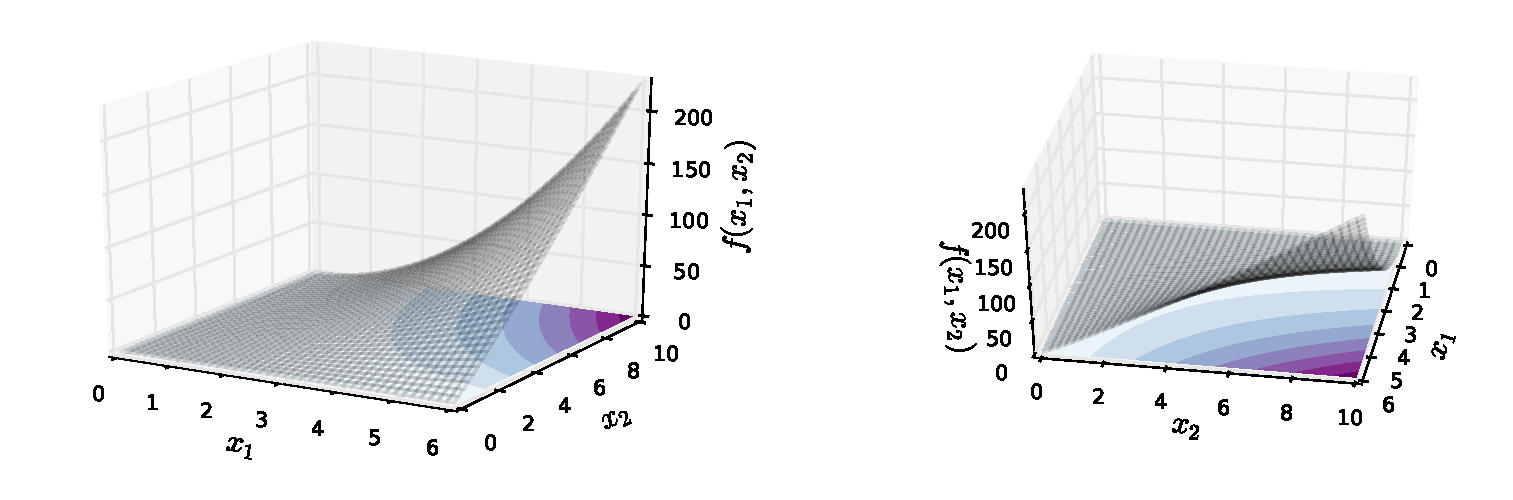
\includegraphics[width=1.0\linewidth]{IRCobbDougcrop}
\end{figure}
\end{frame}

\begin{frame}[fragile]
\frametitle{Quasiconcavity and quasiconvexity}
\framesubtitle{Caveats}
\begin{itemize}
\item A function can be both quasiconcave and quasiconvex. (Consider $ f(x) = x $.)\bigskip
\item As a consequence of the previous property, e.g. a quasiconvex function can be concave (consider $ \ln x $ for $ x \in \mathbb{R}_{++} $).\bigskip
\item The sum of quasiconcave functions is not necessarily quasiconcave.\bigskip
\item A quasiconcave (quasiconvex) function can be discontinuous.
\end{itemize}
\end{frame}

\begin{frame}[fragile]
\frametitle{Sufficient conditions for optimality in concave programs}
By virtue of the structure of concave programs, obtaining sufficiency results for them is more direct:
\begin{Fact}
Let the functions $ f $ and $ g_i,~i=1,\ldots,m $, be defined and continuously differentiable on an open convex set $ U \subseteq \mathbb{R}^n$. Let $ f $ be quasiconcave with non-vanishing gradient and $ g_i $ be quasiconvex on $ U $.
Suppose further that the following constraint qualification, known as \emph{Slater's condition}, is true: \newline There exists a point $ \mathbf{z} \in U $ such that $ g_i(\mathbf{z})<b_i,~i=1,\ldots,m. $

Consider the problem \eqref{eq:objconc}-\eqref{eq:constrconc} and form the Lagrangian in the usual manner as $ \mathcal{L}(\mathbf{x}) = f(\mathbf{x}) - \sum_{i=1}^{m}\lambda_i (g_i(\mathbf{x})-b_i) $. If there exist a feasible point $ \mathbf{x^*} $ and multipliers $ \lambda_1^*,\ldots,\lambda_m^* $ such that \[ \nabla \mathcal{L}(\mathbf{x^*}) = \mathbf{0}, \]
\[ \lambda_i^* \geq 0 \text{ and } \lambda_i^* (g_i(\mathbf{x^*})-b_i) = 0,~i=1,\ldots,m, \]

then $ \mathbf{x^*} $ is a global maximum for the problem \eqref{eq:objconc}-\eqref{eq:constrconc}.
\label{fc:SCsConcaveConstr}
\end{Fact}
\end{frame}

\begin{frame}[fragile]
\frametitle{Comments}
\begin{itemize}
\item If the functions $ g_i $ in Fact \ref{fc:SCsConcaveConstr} are linear, then the result is valid in the absence of Slater's condition.\bigskip
\item The statement of Fact \ref{fc:SCsConcaveConstr} can be weakened slightly by requiring that only the \emph{active} constraints be quasiconvex.
\end{itemize}
\end{frame}

\end{section}
\begin{frame}[fragile]
\frametitle{Readings}
Main references:

Syds\ae{}ter et al. [SHSS] \emph{Further mathematics for economic analysis}. Chapter 3.\bigskip

Additional readings:

Simon and Blume. \emph{Mathematics for economists}. Chapters 18 and 19.

Chiang and Wainwright. \emph{Fundamental methods of mathematical economics}. Chapter 13.
\end{frame}

\end{document}